\chapter{Rancangan, Implementasi, dan Pengujian}

\section{Perancangan Perangkat Lunak}
Subbab perancangan perangkat lunak menjelaskan deskripsi aplikasi, analisis kebutuhan fungsional dan non-fungsional, desain perangkat lunak, serta interaksinya.

	\subsection{Deskripsi Umum Aplikasi}
	Aplikasi pengumpulan data yang dibuat merupakan pengembangan terhadap aplikasi \textit{spreadsheet} kolaboratif yang sudah ada sebelumnya yakni EtherCalc. Aplikasi yang ditambahkan ini yang akan melakukan pengaturan koneksi ke basis data. Saat pengguna menginginkan penyimpanan data ke dalam basis data yang dituju, aplikasi ini akan melakukan pencarian bagian label dan data dan melakukan validasi masukan sebelum memasukkan data ke dalam basis data. 

	\subsection{Spesifikasi Kebutuhan}
	Pada subbab ini akan dipaparkan \textit{use case} aplikasi yang akan dibuat serta kebutuhan fungsional dan non-fungsional dari aplikasi. Kasus penggunaan oleh pengguna diberi ID dengan format UC-XX dengan UC menyatakan \textit{use case} dan XX menyatakan nomor. Pengguna adalah pihak yang menggunakan aplikasi \textit{spreadsheet} yang sudah ditambahkan fitur pengumpulan data. Kasus penggunaan oleh pengguna dijelaskan pada Tabel \ref{KebutuhanPengguna}.

	\begin{longtable}{ | p{2cm} | p{10cm} | }
	    \caption{Kasus Penggunaan oleh Pengguna}
	    \label{KebutuhanPengguna}\\ \hline
	    \centering\bfseries{ID} & \centering\bfseries{Keterangan} \tabularnewline \hline
	    \endfirsthead
	    \hline
	    \centering\bfseries{ID} & \centering\bfseries{Keterangan} \tabularnewline \hline
	    \endhead
	    UC-01 & Pengguna dapat menentukan basis data tujuan dengan konfigurasi basis data yang diinginkan. \\ \hline
	    UC-02 & Pengguna dapat memuat \textit{spreadsheet} serta menyimpan data ke dalam basis data saat dibutuhkan. \\ \hline
	    UC-03 & Pengguna dapat memperbaiki atribut yang terdeteksi secara otomatis. \\ \hline
	    UC-04 & Pengguna dapat memberikan batasan dan validasi pada suatu domain data. \\ \hline
	\end{longtable}

	Berdasarkan kasus penggunaan di atas, dirancang kebutuhan fungsional perangkat lunak yang diberi ID dengan format FR-XX dengan FR merupakan singkatan dari \textit{functional requirement} dan XX menyatakan nomor kebutuhan. Kebutuhan fungsional dijelaskan pada Tabel \ref{KebutuhanFungsional}.

	\begin{longtable}{ | p{2cm} | p{6cm} | p{4cm} | }
	    \caption{Kebutuhan Fungsional Aplikasi}
	    \label{KebutuhanFungsional}\\ \hline
	    \centering\bfseries{ID} & \centering\bfseries{Keterangan} & \centering\bfseries{ID Use Case Terkait} \tabularnewline \hline
	    \endfirsthead
	    \hline
	    \centering\bfseries{ID} & \centering\bfseries{Keterangan} & \centering\bfseries{ID Use Case Terkait} \tabularnewline \hline
	    \endhead
	    FR-01 & Aplikasi dapat melakukan koneksi kepada basis data yang ditentukan oleh pengguna melalui data masukan berupa \textit{host}, \textit{port}, \textit{username}, \textit{password}, dan \textit{database} dari basis data yang dituju. & UC-01 \\ \hline
	    FR-02 & Aplikasi dapat melakukan perintah basis data kepada basis data yang dituju. & UC-01, UC-02 \\ \hline
	    FR-03 & Aplikasi menyediakan tombol untuk melakukan \textit{commit} terhadap data yang akan disimpan. & UC-02 \\ \hline
	    FR-04 & Aplikasi dapat menampilkan hasil identifikasi label dan data & UC-03 \\ \hline
	    FR-05 & Aplikasi menyediakan fitur bagi pengguna agar dapat mengubah hasil identifikasi label dan data & UC-03 \\ \hline
	    FR-06 & Aplikasi menyediakan fitur bagi pengguna agar dapat menambahkan batasan masukan pada suatu data & UC-04 \\ \hline
	    FR-07 & Aplikasi dapat melakukan validasi data masukan sesuai dengan batasan yang diberikan oleh pengguna & UC-04 \\ \hline
	\end{longtable}

	Selain kebutuhan fungsional, dijabarkan juga kebutuhan non-fungsional yang memiliki ID dengan format NF-XX dengan NF merupakan singkatan dari \textit{non-functional requrirement} dan XX menyatakan nomor. Kebutuhan non-fungsional disajikan pada Tabel \ref{KebutuhanNonfungsional}.

	\begin{longtable}{ | p{2cm} | p{6cm} | p{4cm} | }
	    \caption{Kebutuhan Non-fungsional Aplikasi}
	    \label{KebutuhanNonfungsional}\\ \hline
	    \centering\bfseries{ID} & \centering\bfseries{Keterangan} & \centering\bfseries{ID Use Case Terkait} \tabularnewline \hline
	    \endfirsthead
	    \hline
	    \centering\bfseries{ID} & \centering\bfseries{Keterangan} & \centering\bfseries{ID Use Case Terkait} \tabularnewline \hline
	    \endhead
	    NF-01 & Data masukan pengguna disimpan secara persisten. & UC-01, UC-02 \\ \hline
	    NF-02 & Aplikasi dapat berjalan diatas aplikasi \textit{spreadsheet} EtherCalc & - \\ \hline
	\end{longtable}

	\subsection{Kebutuhan Modul} \label{KebutuhanModul}
	Pembangunan fitur ini diatas aplikasi EtherCalc terdiri dari lima buah modul, yaitu:
	\begin{enumerate}
		\item Modul \texttt{player}, bertugas sebagai jembatan antara \textit{front-end} dan \textit{back-end} dari fitur.
		\item Modul \texttt{db}, bertugas untuk antarmuka baca tulis basis data.
		\item Modul \texttt{framefinder}, bertugas untuk mendeteksi secara otomatis bagian label dan data pada tabel.
		\item Modul \texttt{hierarchyfinder}, bertugas untuk mendeteksi secara otomatis tabel-tabel yang ada dalam suatu \textit{sheet}.
		\item Modul \texttt{checker}, bertugas untuk melakukan pengecekan data sebelum diteruskan ke basis data.
	\end{enumerate}

	Ketergantungan antar modul dapat dilihat pada Gambar \ref{ModuleDependency}

	\begin{figure}[htb]
	    \centering
	    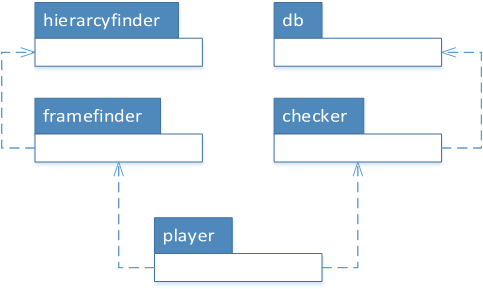
\includegraphics[width=0.6\textwidth]{resources/chapter-4-module-dependecy.png}
	    \caption{Ketergantungan Antar Modul}
		\label{ModuleDependency}
	\end{figure}

	\subsection{Kolaborasi Antar Modul}
	Proses fitur ini akan dilakukan melalui modul \texttt{player} yang dapat menerima perintah pengguna melalui \textit{front-end}. Selanjutnya modul \texttt{framefinder} akan melakukan pendeteksian label dan data secara otomatis pada masing-masing tabel yang terdapat pada \textit{sheet}. Tabel-tabel tersebut didapatkan melalui modul \texttt{hierarchyfinder}. Selanjutnya, pada saat menerima perintah penyimpanan, modul \texttt{checker} akan dipanggil oleh \texttt{player}. Jika data masukan sudah benar, maka modul \texttt{db} akan melakukan pennyimpanan ke dalam basis data. Kolaborasi antar modul disajikan pada Gambar \ref{ModuleFlow}.

	\begin{figure}[htb]
	    \centering
	    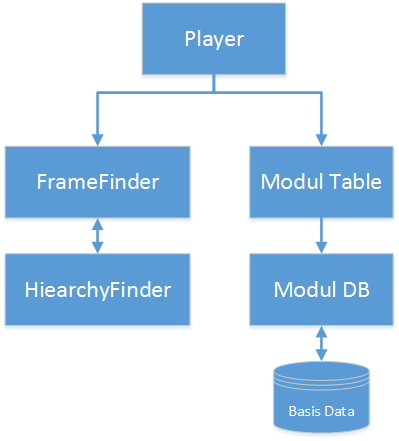
\includegraphics[width=0.4\textwidth]{resources/chapter-4-module-flow.png}
	    \caption{Kolaborasi Antar Modul}
		\label{ModuleFlow}
	\end{figure}


\section{Implementasi}
Implementasi dilakukan dengan membangun modul yang telah dijabarkan pada Subbab \ref{KebutuhanModul} dengan menggunakan bahasa Javascript, menyesuaikan dengan modul lain yang telah ada pada aplikasi EtherCalc.
	\subsection{Modul Player}
	Modul \texttt{player} merupakan modul yang menjembatani masukan pengguna dari yang berasal dari \textit{front-end} sehingga dapat diterima oleh modul yang berada di \textit{back-end}. Modul ini hanya terdiri dari satu kelas utama yakni kelas \texttt{player} yang berisi fungsi-fungsi yang dapat dipanggil oleh \textit{front-end} yang dapat dilihat pada Tabel \ref{FungsiModulPlayer}.

	\begin{longtable}{ | p{2cm} | p{10cm} | }
	    \caption{Fungsi pada Kelas \texttt{Player}}
	    \label{FungsiModulPlayer}\\ \hline
	    \centering\bfseries{Fungsi} & \centering\bfseries{Keterangan} \tabularnewline \hline
	    \endfirsthead
	    \hline
	    \centering\bfseries{Fungsi} & \centering\bfseries{Keterangan} \tabularnewline \hline
	    \endhead
	    refresh & Melakukan pembaharuan tampilan.\\ \hline
	    save & Melakukan pemanggilan terhadap modul \texttt{checker} dan melakukan penyimpanan ke basis data. \\ \hline
	    scan & Melakukan identifikasi tabel melalui pemanggilan modul \texttt{framefinder} yang selanjutnya akan menampilkan hasil identifikasi dan kolom perubahan konfigurasi yang dapat diisi pengguna. \\ \hline
	    saveConfig & Melakukan penyimpanan konfigurasi tabel yang dilakukan oleh pengguna. \\ \hline
	    connect & Melakukan koneksi ke basis data yang dipilih. \\ \hline
	\end{longtable}
	(( jelasin yang menerima input pengguna pake script ))

	\subsection{Modul DB}
	Modul basis data digunakan sebagai antarmuka modul lain untuk melakukan operasi I/O basis data. Pada Tugas Akhir ini, basis data yang digunakan adalah MySQL. Modul ini hanya terdiri dari satu kelas utama yakni kelas \texttt{db}. Kelas ini memiliki tugas sebagai penghubung aplikasi ke basis data MySQL yang dipilih. Fungsi-fungsi yang terdapat pada kelas ini dapat dilihat pada Tabel \ref{FungsiModulDB}.

	\begin{longtable}{ | p{2cm} | p{10cm} | }
	    \caption{Fungsi pada Kelas \texttt{DB}}
	    \label{FungsiModulDB}\\ \hline
	    \centering\bfseries{Fungsi} & \centering\bfseries{Keterangan} \tabularnewline \hline
	    \endfirsthead
	    \hline
	    \centering\bfseries{Fungsi} & \centering\bfseries{Keterangan} \tabularnewline \hline
	    \endhead
	    createTable & Fungsi yang digunakan untuk membuat Table tempat pengisian data.\\ \hline
	    isTableExists & Melakukan pengecekan ada atau tidaknya tabel tersebut pada basis data.\\ \hline
	    dropTable & Menghapus tabel yang dipilih.\\ \hline
	    insertData & Memasukkan data ke dalam tabel yang dipilih.\\ \hline
	\end{longtable}

	Tabel akan dibuat pada basis data yang ditentukan, setiap tabel merepresentasikan suatu tabel pada \textit{spreadsheet} yang ditentukan oleh pengguna. \textit{Header} yang didefinisikan oleh pengguna pada \textit{spreadsheet} akan dijadikan \textit{column} pada tabel basis data, tipe yang dibentuk mengikuti masukan pengguna. Tiap baris data yang ada dibawah \textit{header} pada \textit{spreadsheet} akan ditranslasikan menjadi bentuk relasional agar dapat dimasukan ke dalam tabel.
	
	\subsection{Modul Hierarchyfinder}
	Modul \texttt{hierarchyfinder} menggunakan algoritma \textit{hierarchical clustering} untuk dapat mengetahui mana yang merupakan suatu kesatuan tabel pada suatu \textit{sheet}. Modul ini dapat menentukan tabel-tabel yang terdapat pada suatu \textit{sheet} yang selanjutnya akan dilakukan identifikasi label oleh modul \texttt{framefinder}. Algoritma \textit{hierarchical clustering} yang digunakan menganggap setiap sel pada \textit{spreadsheet} merupakan suatu node. Sel-sel yang bersebelahan dengan sel tersebut akan dianggap tetangga sehingga memiliki jarak sama dengan 0. Sel yang digabungkan dengan sel lain akan dihitung sebagai satu \textit{node}. Aturan perhitungan jarak antar \textit{node} dapat dilihat pada kode di Kode \ref{KodeJarak}.\\

	\begin{lstlisting}[frame=single, basicstyle=\linespread{1}\scriptsize\listingsfont, captionpos=b, caption={Perhitungan Jarak \textit{Node}}, label=KodeJarak]
	# Fungsi cellDistance(v1, v2)
	# Parameter pada fungsi adalah v1 (node 1) dan v2 (node 2)
	t = new Table null, null
	colD = t.GetCellCol(v1[0]) - t.GetCellCol(v2[0])
	rowD = t.GetCellRow(v1[0]) - t.GetCellRow(v2[0])

	# Jika sel saling bertetangga tetapi bukan secara diagonal
	# Jika bertetangga, jarak kedua sel adalah 0
	if colD == 0
		if rowD == 1 or rowD == -1
			return 0
	if rowD == 0
		if colD == 1 or colD == -1
			return 0

	# Jika tidak, cek apakah sel bertetangga secara diagonal
	# Jika bertetangga, jarak kedua sel adalah 0
	leftTop = [[v1[1], v1[2]], [v2[1], v2[2]]]
	leftBot = [[v1[1], (v1[2] + v1[4])], [v2[1], (v2[2] + v2[4])]]
	righTop = [[(v1[1] + v1[3]), v1[2]], [(v2[1] + v2[3]), v2[2]]]
	righBot = [[(v1[1] + v1[3]), (v1[2] + v1[4])], [(v2[1] + v2[3]), (v2[2] + v2[4])]]

	if (leftTop[0][0] == righTop[1][0] and leftTop[0][1] == righTop[1][1])
		return 0
	if (leftBot[0][0] == righBot[1][0] and leftBot[0][1] == righBot[1][1])
		return 0

	if (leftTop[1][0] == righTop[0][0] and leftTop[1][1] == righTop[0][1])
		return 0
	if (leftBot[1][0] == righBot[0][0] and leftBot[1][1] == righBot[0][1])
		return 0

	if (leftTop[0][0] == leftBot[1][0] and leftTop[0][1] == leftBot[1][1])
		return 0
	if (righTop[0][0] == righBot[1][0] and righTop[0][1] == righBot[1][1])
		return 0

	if (leftTop[1][0] == leftBot[0][0] and leftTop[1][1] == leftBot[0][1])
		return 0
	if (righTop[1][0] == righBot[0][0] and righTop[1][1] == righBot[0][1])
		return 0

	# Jika tidak juga, hitung jarak menggunakan teknik Euclidian
	dist = Math.sqrt(Math.pow((v2[1] + (v2[3]/2)) - (v1[1] + (v1[3]/2)), 2) + Math.pow((v2[2] + (v2[4]/2)) - (v1[2] + (v1[4]/2)), 2));
	return dist
	\end{lstlisting}

	Hasil dari pengelompokan ini berupa kelompok-kelompok tabel pada \textit{spreadsheet}. Setiap tabel yang teridentifikasi selanjutnya akan dicari bagian \textit{header} dan \textit{label} menggunakan modul \texttt{framefinder}.

	\subsection{Modul Framefinder}
	Modul \texttt{framefinder} melakukan pengidentifikasian terhadap tabel yang ada sehingga dapat diketahui baris yang merupakan \textit{header} dan \textit{data}. Implementasi modul ini dilakukan dengan mengikuti implementasi yang dilakukan pada penelitian yang dilakukan oleh Chen \citep{Chen2013}. (Jelasin detil dikit implementasinya)

	\subsection{Modul Checker}
	Modul \texttt{checker} memiliki tugas untuk melakukan pengecekan terhadap masukan pengguna pada konfigurasi serta melakukan pengecekan kesesuaian nilai masukan berdasarkan tipe, \textit{range}, serta relasi yang ditentukan oleh pengguna. Jika seluruh kriteria telah dipenuhi, maka modul ini akan memanggil modul \texttt{db} untuk melakukan penyimpanan data. (Jelasin checkingnya)

\section{Pengujian}
% \blindtext

\section{Pembahasan}
% \blindtext